
\label{ch:theory}
\chapter{The Standard Model of Particle Physics}
\label{SM chapter}
\section{Introduction}
By determining the dynamics of the most elementary degrees of freedom, particle physics hopes to uncover the fundamental laws of the universe. The definition of elementary has evolved through time and currently refers to matter and force mediating particles: fermions and bosons, respectively. The Standard Model of Particle Physics (SM) describes the quantum behavior of three of the four fundamental forces: weak, strong, and electromagnetic, via boson and fermion interactions. Gravity is not included in the SM and still under investigation. 
\section{Quantum Field Theory}
In the SM, forces (and particles) are represented as fields. In this context, fields are mathematical objects that define a tensor (e.g. scalar, vector, etc)  at every point on a manifold, here the manifold is space-time. These fields obey laws dictated by Quantum Field Theory (QFT). Particles arise naturally in QFT as quantizied field excitations localized in spacetime. 

According to Noether's theorem, symmetries of a field give rise to conserved quantities (e.g. time-translation invariance leads to energy conservation).  Often in the history of physics, a conserved quantity of a field is found and then the underlying symmetry of the field is inferred. Gauge symmetries are symmetries among the internal degrees of freedom of the field (components of the tensor), which give rise to quantities associated with fields. By specifying the symmetries of a system the dynamics and conserved quantities of the system may be succinctly defined.
\section{$U(1)_{EM}$ Local Gauge Invariance}
The Lagrangian of Quantum Electrodynamics (QED) describes the electromagnetic force. QED may be derived by requiring local $U(1)_{EM}$ gauge invariance of the free dirac fermion Lagrangian, $\psi$:
\begin{equation}
\mathcal{L} = i\bar{\psi}\gamma^{\mu}\partial_{\mu}\psi - m\bar{\psi}{\psi}
\end{equation}
This symmetry may be represented as a complex number with unit modulus, $e^{i\theta}$. U(1) gauge invariance requries this gauge transformation of $\psi$ will leave the Lagrangian unchanged.

\begin{equation}
\psi(x) \rightarrow \psi'(x) = e^{i\theta(x)}\psi(x)
\end{equation}

NB: This transformation is a local gauge transformation as $\theta$ depends on the spacetime coordinate.

By requiring this symmetry of the free Dirac fermion Lagrangian:

\begin{equation}
\mathcal{L} = i\bar{\psi}\gamma^{\mu}\partial_{\mu}\psi - m \bar{\psi}\psi
\end{equation}

The mass term is unaffected, but the kinetic term is modified due to $\theta(x)$.
\begin{equation}
\mathcal{L} \rightarrow \mathcal{L}' = i\bar{\psi} e^{-i\theta(x)}\gamma^{\mu}\partial_{\mu}\psi e^{i\theta(x)} - m \bar{\psi}e^{-i\theta(x)}\psi e^{i\theta(x)}
\end{equation}
\begin{equation}
= i\psi \gamma^{\mu}(\partial_{ \mu }\psi + i \psi \partial_{ \mu } \theta)- m \bar{ \psi } \psi
\end{equation}

The $\partial_{\mu}\theta$ terms breaks the gauge invariance of the Lagrangian. By introducing a new field, $A_{\mu}$ we can recover the gauge invariance of the derivative. Now redefining the derivative as the covariant derivative:

\begin{equation}
D_{\mu}\psi \equiv (\partial_{\mu} - iqA_{\mu})\psi
\end{equation}

And letting $A_{\mu}$ transform under U(1) as:
\begin{equation}
A_{\mu} \rightarrow A_{\mu} +  \delta A_{\mu} 
\end{equation}

The transformed covariant derivative becomes:

\begin{equation}
D_{\mu}\psi \rightarrow D_{\mu}\psi' =  (\partial_{\mu} - iq A_{\mu})\psi'
\end{equation}
\begin{equation}
=  (\partial_{\mu} - iq(A_{\mu} +  \delta A_{\mu} ))\psi e^{i\theta}
\end{equation}
\begin{equation}
=  e^{i\theta}D_{\mu}+ie^{i\theta}\psi(\partial_{\mu}\theta - q\delta A_{\mu}))
 \end{equation}


The covariant derivative can be made gauage invariant by setting the last term to zero.

\begin{equation}
\delta A_{\mu} = \frac{1}{q}\partial_{\mu}\theta
\end{equation}

So now $A_{\mu}$ transforms as:

\begin{equation}
A_{\mu} \rightarrow A_{\mu} + \frac{1}{q}\partial_{\mu}\theta
\end{equation}

Finally, replacing the derivative with the covariant derivative the Dirac Lagrangian we have:

\begin{equation}
\mathcal{L} = i \bar{\psi}\gamma^{\mu}D_{\mu}\psi - m\bar{\psi}\psi - \frac{1}{4}F_{\mu\nu}F^{\mu\nu}
\end{equation}
\begin{equation}
=\mathcal{L}_{QED}
\end{equation}

Here $F_{\mu\nu}\equiv \partial_{\mu}A_{\nu} - \partial_{\nu}A_{\mu}$. This last term in the Lagrangian is the kinetic energy of the gauge boson field.

So we have derived the QED Lagrangian. By requiring the free Dirac Lagrangian to be invariant under local U(1) transformations we have generated a new gauge boson field, $A_{\mu}$, which describes the photon. As expected the photon interacts with fermions.  

Stepping back, a global U(1) gauge symmetry of the free Dirac Lagrangian implies we cannot measure the absolute phase of a charged particle. A local U(1) gauge symmetry changes the phase of fields differently across space time. For this type of transformation to leave the Lagrangian invariant, we had to introduce an additional field, $A_{\mu}$, which "communicates" these phase changes across space-time. In less formal language this effectively means: if the field at one location changes, this change is conferred to other particles via $A_{\mu}$.

\section{Yang-Mills Gauge Theories}
Requiring $U(1)_{EM}$ gauge invariance of the free Dirac Lagrangian gave us QED. Requiring different gauge symmetries we can derive the structure of other interactions. Any gauge symmetry may be written as:

\begin{equation}
\psi_{i} \rightarrow \exp(i\theta^{a}T^{a}_{ij})\psi_{j}
\end{equation}

Here $\theta$ is a dimensionless real parameter and T is the generator of the gauge symmetry group. With this the covariant derivative can be written as:

\begin{equation}
D_{\mu}\psi_{i} \equiv \partial_{\mu}\psi_{i} + igA^{a}_{\mu}T^{a}_{ij}\psi_{j}
\end{equation}

Then the gauge field must transform as:

\begin{equation}
A^{a}_{\mu} \rightarrow A^{a}_{\mu} - \frac{1}{g}\partial_{\mu}\theta^{a} - f^{abc} \theta^{b} A_{\mu}^{c}
\end{equation}

Here f is the structure constant of the gauge group. The field strength tensor is given by:

\begin{equation}
F^{a}_{\mu\nu} \equiv \partial_{\mu}A^{a}_{\nu} - \partial_{\nu}A^{a}_{\mu} - gf^{abc}A^{b}_{\mu}A^{c}_{\nu}
\end{equation}
\begin{equation}
F^{a}_{\mu\nu} \rightarrow F^{a}_{\mu\nu} - f^{abc} \theta^{b}F^{c}_{\mu\nu}
\end{equation}

This gives the Yang-Mills Lagrangian:
\begin{equation}
\mathcal{L}_{YM}= -\frac{1}{4}F^{a\mu\nu}F^{a}_{\mu\nu}+i\bar{\psi_{i}}\gamma^{\mu}D_{\mu}\psi_{i}+m\bar{\psi_{i}\psi_{i}}
\end{equation}
\section{Particles in the Standard Model}
The SM consists of fermions (half-interger spin matter constituents) and bosons (integer spin force meditators). Fermions are spinor representations of the Poincare group and can be further separated into leptons and quarks. Bosons are the result of requiring a particular symmetry among the spinor fields:

\begin{equation}
SU(3)_{C} \times SU(2)_{L} \times U(1)_{Y}
\end{equation}

$SU(3)_{C}$ is the symmetry group of the strong force and generates eight gluon fields, $G_{\mu}$. $SU(2)_{L}$ is the symmetry group of the Electroweak force and generates three electroweak boson fields. The mixing of this $SU(2)_{L}$ and $U(1)_{Y}$ gives rise to the photon field, where Y is the weak-hypercharge:

\begin{equation}
Y= 2(Q-T_{3})
\end{equation}

Q is the electromagnetic charge, and $ T_{3}$ is the z-component of the weak isospin. Weak isospin is the charge associated with the $SU(2)_{L}$ symmetry. The corresponding covariant derivative is then:

\begin{equation}
D_{\mu}\phi \equiv (\partial_{\mu} + ig_{1}B_{\mu}Y_{L/R} + [ig_{2}W^{\alpha}_{\mu}T^{\alpha}]_{L} + [ig_{3}G^{\alpha}_{\mu}\tau^{\alpha}]_{C})\psi
\end{equation}

It is important to note that the gauge symmetry of the SM yields a particular structure of the fermion representations. So for a given fermion to interact with a given gauge field it must have a non-zero corresponding Noether charge for that gauge symmetry. If the corresponding Noether charge is zero, that fermion transforms as a singlet and does not participate in that gauge interaction. 

Fermions are divided into quarks and leptons based on their transformations under $SU(3)_{C}$. Quarks transform as color triplets. Leptons transform as color singlets and consequently do not interact with gluons. 
Fermions may be further classified by their $SU(2)_{L}$ interactions. Only the left-chiral part of fermions (denoted by L here) transform as $SU(2)_{L}$ doublets, the right-chiral part forms singlets under this gauge. Lastly, all these groups of particles come in three generations, each a heavier copy of the previous, but with differing flavor quantum numbers. This is summarized in Table ~\ref{tbl:SMparticles} and shown in Figures ~\ref{fig:sm_particles} and \ref{fig:sm_particle_interactions}.

\begin{table}[!hbt]
  \resizebox{\textwidth}{!}{\begin{tabular}{|l|c|c|c|c|}
    \hline
    SM Fermion Gauge Group & First Generation & Second Generation & Third Generation & $(SU(3)_{C}, SU(2)_{L},U(1)_{Y})$ Representations \\ 
    \hline
    \hline
    Left-handed quarks & $\begin{pmatrix} u_{L}^{r} & u_{L}^{g} & u_{L}^{b} \\d_{L}^{r} & d_{L}^{g} & d_{L}^{b} \end{pmatrix}$ & $\begin{pmatrix} c_{L}^{r} & c_{L}^{g} & c_{L}^{b} \\s_{L}^{r} & s_{L}^{g} & s_{L}^{b} \end{pmatrix}$ & $\begin{pmatrix} t_{L}^{r} & t_{L}^{g} & t_{L}^{b} \\b_{L}^{r} & b_{L}^{g} & b_{L}^{b} \end{pmatrix}$ & $(3,2,\frac{1}{6})$ \\
    \hline
    
    Right-handed quarks & $( u_{R}^{r}, u_{R}^{g}, u_{R}^{b})$ & $(c_{R}^{r}, c_{R}^{g}, c_{R}^{b})$ & $(t_{R}^{r}, t_{R}^{g}, t_{R}^{b})$ & $(3,1,\frac{2}{3})$ \\
    & $( d_{R}^{r}, d_{R}^{g}, d_{R}^{b})$ & $(s_{R}^{r}, s_{R}^{g}, s_{R}^{b})$ & $(b_{R}^{r}, b_{R}^{g}, b_{R}^{b})$ & $(3,1,-\frac{1}{3})$ \\
    \hline
    Left-handed leptons & $\begin{pmatrix} \nu_{e}^{L}  \\ e_{L} \end{pmatrix}$ &$\begin{pmatrix} \mu_{e}^{L}  \\ \mu_{L} \end{pmatrix}$ & $\begin{pmatrix} \tau_{e}^{L}  \\ \tau_{L} \end{pmatrix}$ & $(1,2,-\frac{1}{2})$ \\
    \hline
    Right-handed leptons & $e_{R}$ & $\mu_{R}$ & $\tau_{R}$ & $(1,1,-1)$ \\
    \hline
\end{tabular}}
  \caption{Representations of the SM fermions under $SU(3)_{C}\times SU(2)_{L} \times U(1)_{Y}$ gauge symmetry group. Rows are correspond to different weak isospin states and columns to different QCD color states.}
  \label{tbl:SMparticles}
\end{table}

\begin{figure}[h!]
  \centering
  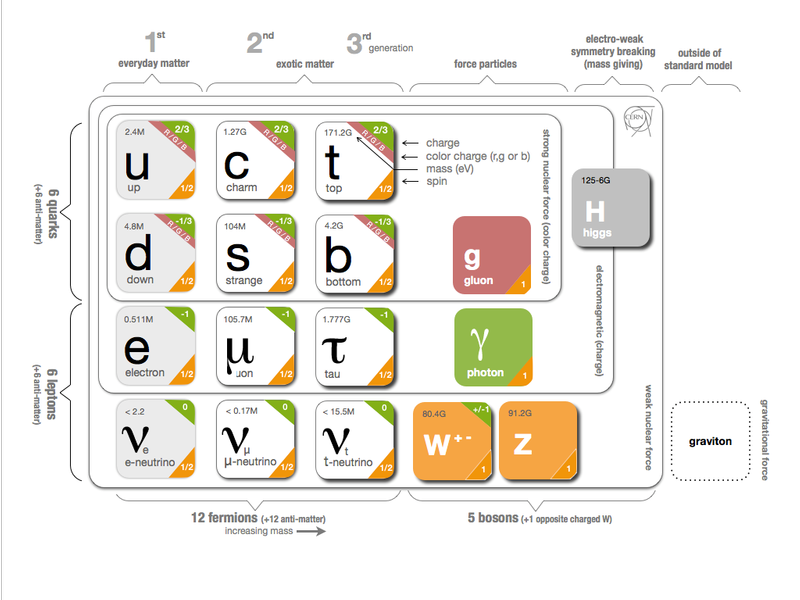
\includegraphics[width=\hsize]{figures/theory/particles.png}
  \caption{The particles of the Standard Model.} 
  \label{fig:sm_particles}
\end{figure}
\FloatBarrier

\begin{figure}[h!]
  \centering
  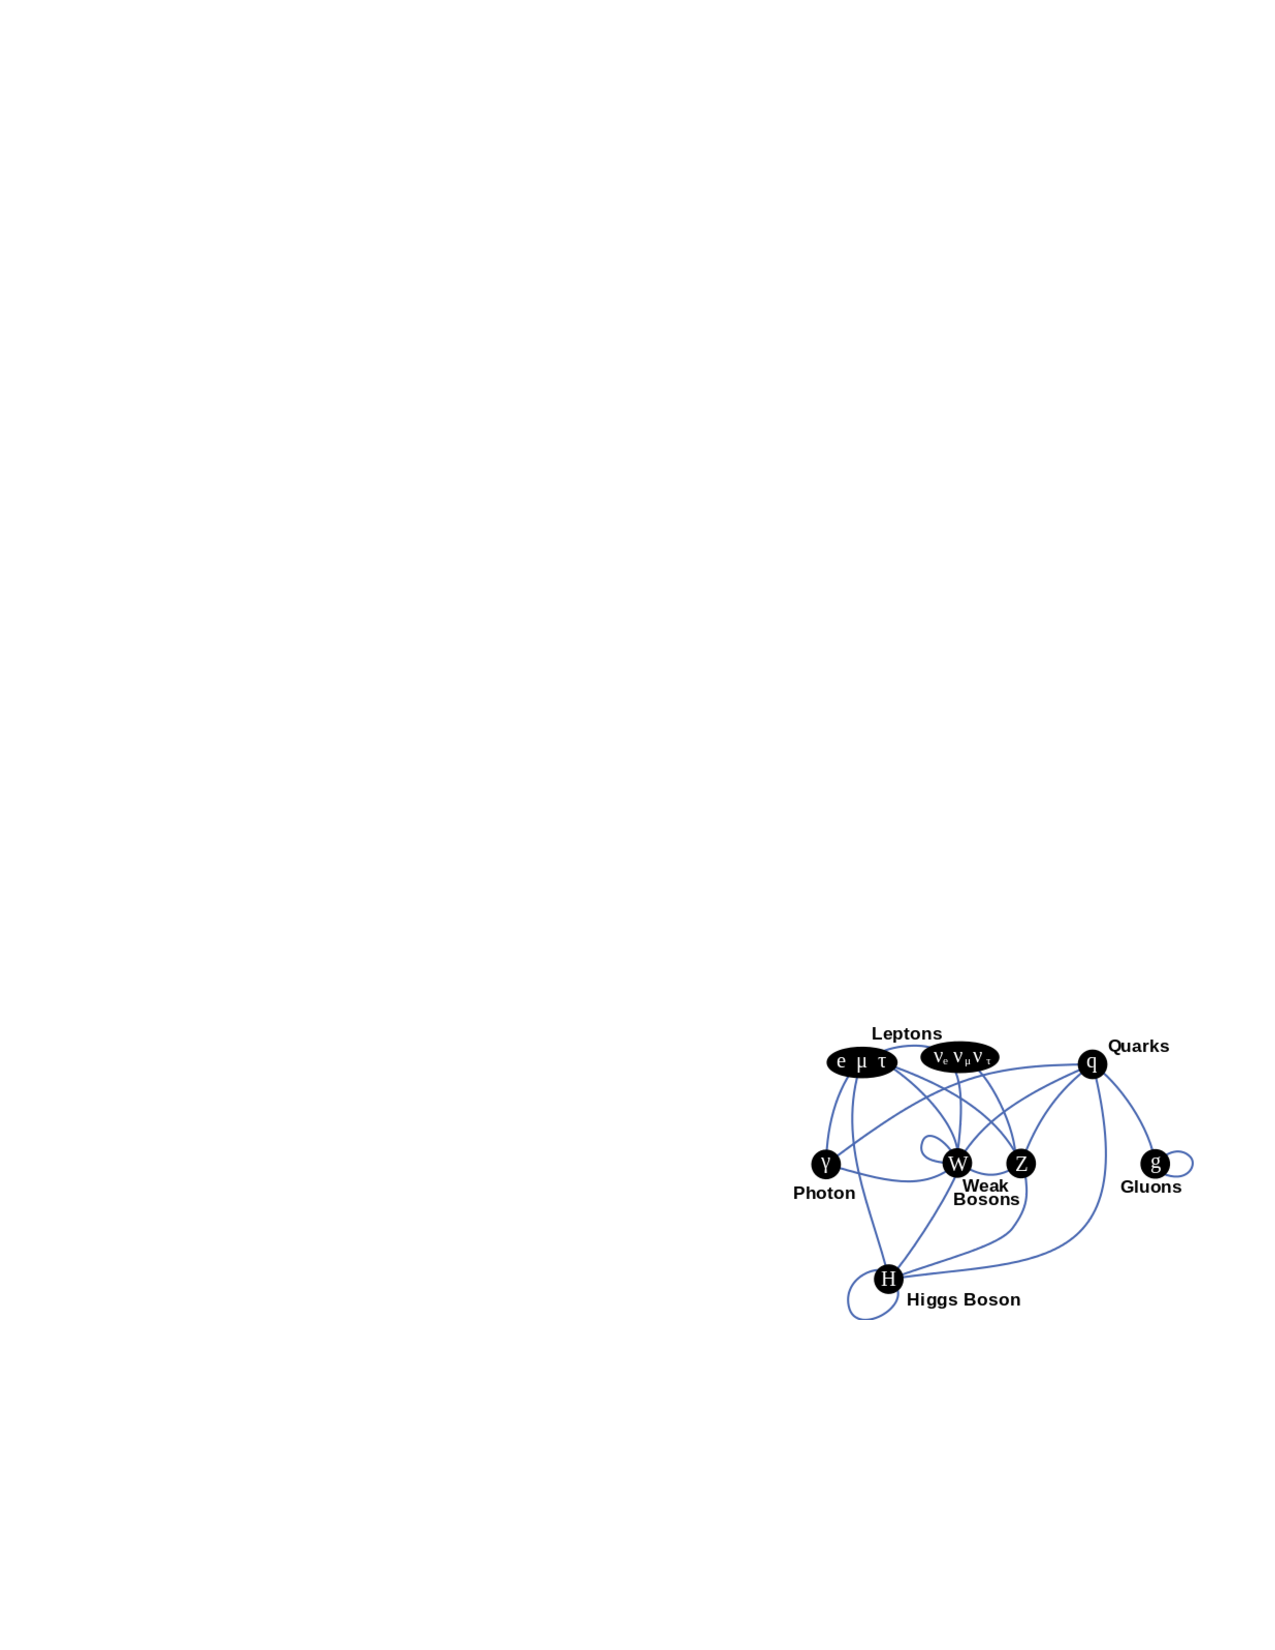
\includegraphics[width=\hsize]{figures/theory/particle_interactions.pdf}
  \caption{Summary of how Standard Model particles interact with other Standard Model particles.} 
  \label{fig:sm_particle_interactions}
\end{figure}
\FloatBarrier


Now we can understand the SM Lagrangian density as a Yang-Mills theory with the gauge group: $SU(3)_{C}\times SU(2)_{L} \times U(1)_{Y}$ with an additional $SU(2)$ complex scalar Higgs field doublet that will be discussed later.


\begin{flalign}\nonumber
\mathcal{L} _{SM} &= \underbrace{-\frac{1}{4}B_{\mu\nu}B^{\mu\nu}-\frac{1}{4}W^{a}_{\mu\nu}W^{a\mu\nu}-\frac{1}{4}G^{\alpha}_{\mu\nu}G^{\alpha\mu\nu}}_\text{Kinetic Energies and Self-Interactions of Gauge Bosons}&&\\\nonumber
&+\underbrace{\bar{L_{i}}\gamma^{\mu}(i\partial_{\mu}-\frac{1}{2}g_{1}Y_{iL}B_{\mu}-\frac{1}{2}g_{2}\sigma^{a}W_{\mu}^{a})L_{i}}_\text{Kinetic Energies and EW Interactions of Left-handed Fermions}&&\\\nonumber
&+\underbrace{\bar{R_{i}}\gamma^{\mu}(i\partial_{\mu}-\frac{1}{2}g_{1}Y_{iR}B_{\mu})R_{i}}_\text{Kinetic Energies and EW Interactions of Right-Handed Fermions}&&\\\nonumber
&+\underbrace{\frac{ig_{3}}{2}\bar{Q_{j}}\gamma^{\mu}\lambda^{\alpha}G^{\alpha}_{\mu}Q_{j}}_\text{Strong Interactions between Quarks and Gluons}&&\\\nonumber
&+\underbrace{\frac{1}{2}|(i\partial_{\mu}-\frac{1}{2}g_{1}B_{\mu}-\frac{1}{2}g_{2}\sigma^{a}W_{\mu}^{a})\Phi|^{2} - V(\Phi)}_\text{Electroweak Boson Masses and Higgs Couplings}&&\\\nonumber
&-(\underbrace{y^{d}_{kl}\bar{L_{k}}\Phi R_{l}+y^{u}_{kl}\bar{R_{k}}\widetilde{\Phi}L_{l}+h.c.)}_\text{Fermion Mass terms and Higgs Couplings}&&\\\nonumber
\end{flalign}

Here several abstract spaces are being spanned:
\begin{itemize}
\item[--]a spans the three $SU(2)_{L}$ gauge fields with generators expanded in Pauli matrics, $T^{\alpha}=\frac{1}{2}\sigma^{a}$
\item[--]$\alpha$ spans the eight $SU(3)_{C}$ gauge fields, with generators expanded in Gell-Mann matrices, $\tau^{\alpha}=\frac{1}{2}\lambda^{\alpha}$
\item[--]L/R represent left and right projections of Dirac fermion fields. The Strong interaction is not chiral, so Q = L+R
\item[--]$\mu$ and $\nu$ are four-vector indices
\item[--]i, j, k are summed over the three generations of SM particles. 
\end{itemize}

\section{Higgs Mechanism}
The SM Lagrangian without the addition of a Higgs field does not allow for gauge boson and fermion mass terms: $\frac{1}{2}m_{A}^{2}A_{\mu}A_{\mu}$ and $m(\bar{\psi}\psi)$,  as these terms are not gauge invariant. By introducing the Higgs field, mass terms for these particles may be included in a gauge invariant way. This field is a complex doublet with a potential $V(\Phi)$:

\begin{equation}
\Psi = \begin{pmatrix} \Phi^{\dagger} \\ \Phi^{0} \end{pmatrix}
\end{equation}
\begin{equation}
V(\Phi)=\mu^{2}\Phi^{\dagger}\Phi + \lambda |\Phi^{\dagger}\Phi|^{2}
\end{equation}

The minima of this field occurs for $|\Phi|= \sqrt{\frac{\mu^{2}}{2\lambda}} \equiv \frac{v}{2}$. This yields degenerate minima, this symmetry is broken by choosing a specific minima (a.k.a. spontaneous symmetry breaking). By convention  $\Phi_{min} = \frac{1}{\sqrt{2}}\begin{pmatrix}0 \\ v \end{pmatrix}$ is chosen. This means the ground state of the Higgs field (Higgs vacuum) is non-zero, $\sqrt{\frac{-\mu^{2}}{\lambda}}$. The Higgs Field may now be expanded around this new ground state:

\begin{equation}
\Phi(x)=\frac{1}{\sqrt{2}}\begin{pmatrix} 0 \\ v+h(x)\end{pmatrix}
\end{equation}

This non-zero Higgs vacuum now generates mass terms for the gauge bosons from the following term in the Lagrangian:

\begin{equation}
|(-\frac{1}{2}g_{1}B_{\mu}-\frac{1}{2}g_{2}\sigma^{a}W_{\mu}^{a})\Phi|^{2}=\frac{1}{2}m_{W}^{2}W_{\mu}^{+}W^{-\mu}+\frac{1}{2}m_{Z}^{2}Z_{\mu}Z^{\mu}
\end{equation}

where:
\begin{equation}
W^{\pm}_{\mu} \equiv \frac{1}{\sqrt{2}}(W^{1}_{\mu} \mp iW^{2}_{\mu})
\end{equation}
\begin{equation}
Z_{\mu} \equiv \frac{1}{\sqrt{g_{1}^{2}+g_{2}^{2}}}(g_{2}W^{2}_{\mu}-g_{1}B_{\mu})
\end{equation}
\begin{equation}
m_{W} = \frac{vg_{2}}{\sqrt{2}}
\end{equation}
\begin{equation}
m_{Z} = \frac{v}{\sqrt{2}}\sqrt{g_{1}^{2} + g_{2}^{2}}
\end{equation}

The Higgs field also generates a mass term for the Higgs boson and self-interactions for the Higgs boson. 
\section{Electroweak Theory}
$SU(2)_{L}$ generates $W^{\pm}, W^{0}$ gauge bosons, which would be massless if $SU(2)_{L}$ was a perfect symmetry. These bosons are massive as this symmetry is broken. The mass eigenstates, Z and $\gamma$ given by: 
\begin{equation}
\begin{pmatrix} Z_{\mu} \\ A_{\mu} \end{pmatrix} = \begin{pmatrix} \cos \theta_{W} & -\sin \theta_{W} \\ \sin \theta_{W} & \cos \theta_{W} \end{pmatrix} \begin{pmatrix} W^{3}_{\mu} \\ B_{\mu} \end{pmatrix}
\end{equation} 

Here $\theta_{W}$ is the Weinberg angle given by: 
\begin{equation}
\cos\theta_{W}=\frac{g_{2}}{\sqrt{g_{1}^{2}+g_{2}^{2}}} = \frac{m_{W}}{m_{Z}}
\end{equation}
\section{Quantum Chromodynamics}
As mentioned earlier the Strong Force, which binds the proton together, is mediated by gluons. Quantum Chromodynamics is the QFT which describes the interactions of quarks and gluons via $SU(3)_C$ symmetry. QCD contains features not present in Electroweak Interactions due to $SU(3)_C$ generators not commuting (a.k.a. $SU(3)_C$ is a non-abelian group) and the number of quark flavors ($n_{f}$). For example, in QCD there is color confinement and asymptotic freedom due to the structure constants being non-zero. Requiring $SU(3)_C$ local gauge invariance implies:

\begin{equation}
\psi(x) \rightarrow \psi(x)^{'} = \exp[ig_{S}\alpha(x)\cdot\hat{T}]\psi(x)
\end{equation}

where $\alpha(x)$ is the local phase function, $g_{S}$ is the strong coupling constant, and $\hat{T}$ are the eight generators of $SU(3)$ (note $\hat{T^{a}}=\frac{1}{2}\lambda^{a} a$, where $\lambda^{a}$ are the Gell-Mann matrices). As the Gell-Mann matrices are 3x3, this means $\psi$ has three degrees of freedom under these $SU(3)$ rotations. So we represent $\psi$ under $SU(3)$ rotations as:

\begin{equation}
\psi = \begin{pmatrix} \psi_{red} \\ \psi_{green} \\ \psi_{blue}\end{pmatrix}
\end{equation}

Consequently, particle fields transforming under $SU(3)$ rotations have three components which physicists describe as color components (red, green, and blue). A particle's corresponding antiparticle has the corresponding anticolor. This color is the "charge" of QCD and is conserved under $SU(3)$ rotations. Combining colors, color neutral states (e.g. red and antired, or red, green and blue) may be created.
For the free Dirac Lagrangian to remain invariant under $SU(3)$ transformations, we must again postulate a boson field that modifies the derivative. The gluon field tensor is given by ($\alpha=1,...,8)$:

\begin{equation}
G_{\mu\nu}^{k}  = \partial^{\mu}G^{\nu}_{\alpha}-\partial^{\nu}G^{\mu}_{\alpha}-g_{S}f^{\alpha\beta\gamma}G^{\mu}_{\beta}G^{\nu}_{\gamma}
\end{equation}

Here $f^{\alpha\beta\gamma}$ are the structure constants of $SU(3)$. Combining all this gives the QCD Lagrangian:

\begin{equation}
\mathcal{L}_{QCD} = \bar{\psi_{qi}}i\gamma^{\mu} (D_{\mu})_{ij}\psi^{qj} - m\bar{\psi^{qi}}\psi_{qi} - \frac{1}{4}G^{\alpha}_{\mu\nu}G^{\alpha\mu\nu} 
\end{equation}

Here i are the color indicies, and q are the quark flavors. It is important to note that quarks transform under the fundamental representation of $SU(3)$, while gluons transform under the adjoint representation. This means quarks carry a single color charge (red, green, blue, antired, antigreen, antiblue) and gluons carry a color and anticolor charge. 

Figure \ref{fig:QCDinteractions} shows the three dominant QCD interactions. Sincle gluons carry color charge, they interact with one another. This does not occur in QED, as photons do not have electric charge and therefore do not interact with each other. In QED, a bare electron's effective charge is largest closest to the electron and decreases as a function of distance. This is because the QED vacuum fills with particle antiparticle pairs spontaneously, which screen the charge of the bare electron. The larger the distance from the electron, the smaller the effective charge and therefore the weaker the force. 

\begin{figure}[h!]
  \centering
  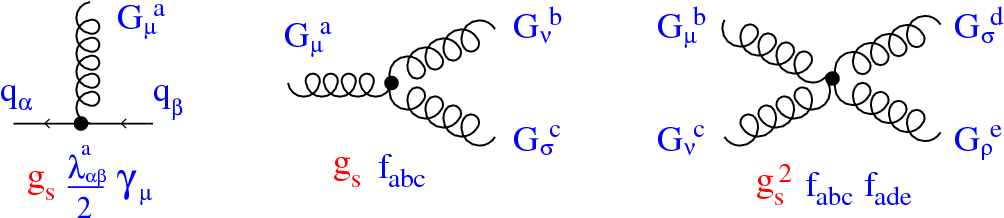
\includegraphics[width=\hsize]{figures/Theory/QCD_vertices.png}
  \caption{This figure shows the three dominant QCD interactions \cite{pich}}f. 
  \label{fig:QCDinteractions}
\end{figure}
\FloatBarrier


As the distance from a quark increases it's effective color charge increases due to the vacuum polarization in QCD. Color charge grows as the distance from the source increases (a.k.a. color is anti-screened in QCD).  In this way, strong interactions become stronger at large distances (low momenta interactions).  At small distances (large momenta interactions) strong interactions are significantly weaker and considered nearly free. This effect of referred to as asymptotic freedom. At large distances, a quark's effective charge is large and the strong force is more significant. This force becomes so strong that quarks form colorless bound states instead of remaining free particles. This effect is known as color confinement. This running of all SM fields is shown in Figure ~\ref{fig:sm_couplings}. 

\begin{figure}[h!]
  \centering
  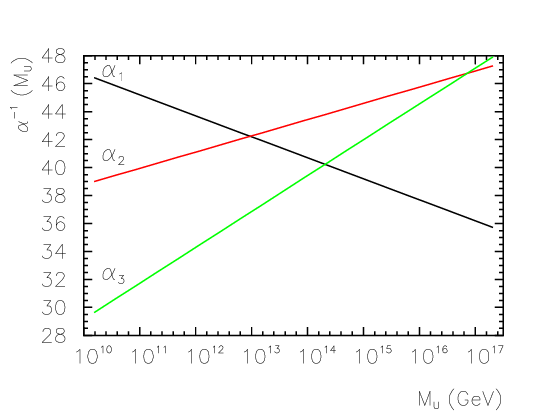
\includegraphics[width=\hsize]{figures/Theory/runningcouplings.png}
  \caption{Strength of the $U(1)$, $SU(2)$, and $SU(3)$ gauge couplings as a function of the energy scale of the interaction (Q). From Ref. \cite{runningcouplings}}. 
  \label{fig:sm_couplings}
\end{figure}
\FloatBarrier


Commonly the change in a particle's effective charge under a given force is quantified with  $\beta(r) \equiv \frac{-de(r)}{d\ln r}$, where e(r) is the effective charge of a given particle under a force. In QED this function is positive but in QCD this function is negative leading to confinement and asymptotic freedom. Moreover, one can calculate how the coupling ($\alpha$) of a force varies with energies. More deeply this amounts to incorporating renormalization and vacuum polarization in the boson propagators. For QCD this is:

\begin{equation}
\alpha_{S}(Q^{2}) = \frac{ \alpha_{s}(\mu^{2}) } { 1+ \frac{ \alpha_{s}( \mu^{2} ) } { 12\pi } ( 33-2n_{f} ) ln( Q^{2}/\mu^{2})}  
\end{equation}


where $Q$ is the momentum of the the force is probed at, $\mu^{2}$ is the renormalization scale, $n_{f}$ is the number of quark flavors. There are six quark flavors in SM QCD, making $33-2n_{f} > 0$. This factor being positive and the $ln(Q^{2}/\mu^{2})$  being in the denominator means that as $Q^{2}$ increases $\alpha_{s}$ decreases. So for large $Q^{2}$, $\alpha_{s}$ is small and SM QCD is asymptotically free, while for small $Q^{2}$, $\alpha_{s}$ is large and SM QCD is confined, as mentioned earlier. 

As stated previously, quarks and gluons have not been observed in isolation. Instead they form bound colorless states. Hadronization is the process by which quarks and gluons form hadrons. The process of hadronization is still an active area of research. One qualitative description is show in Figure \ref{fig:colorstring}. In this figure, as two quarks separate the color field between them is restricted to a tube with energy density of ~1 GeV/fm. As they separate further, the energy in the color field increases, until there is enough energy to produce $q\bar{q}$ pairs, which breaks the color field. This process repeats until quarks and antiquarks have low enough energy to form colorless hadrons. The resulting spray of hadrons is called a jet.

Since quarks and gluons carry different color charges, their respective jets have different properties. As quarks carry only a single color charge (vs. gluons which have color and anticolor charge), so their jets have less constituent particles. More precisely, the Altarelli-Parisi splitting functions ~\cite{altarelli} contain a factor $C_{A}$ for gluon radiation off a gluon and $C_{F}$ for gluon radiation off a quark ($C_{A}/C_{F} = 9/4$). These color factors are the prefactor in the Feynman diagrams for these processes ~\cite{colorfactor}, which leads to gluon jets having more constituents and therefore more tracks than quark jets. Gluon jets also tend to have a larger radius with lower momentum constituents than quarks. There are many novel techniques to distinguish quarks from gluons. For this study the number of charged particles will be focused on.  

\begin{figure}[h!]
  \centering
  \includegraphics[width=\hsize]{figures/Theory/color_string.pdf}
  \caption{A cartoon of string breaking: the QCD string spanned between quark Q and antiquark $\bar{Q}$ breaks due to $q\bar{q}$ creation \cite{colorstring}}.
  \label{fig:colorstring}
\end{figure}
\FloatBarrier

\chapter{Standard Model Successes and Limitations}
The Standard Model has accurately described most of the underlying principles of nature. It has predicted cross sections for strong and electroweak processes that span over ten orders of magnitude correctly, as shown in Figure \ref{fig:SM cross sections}, and contains no known logical inconsistencies. Despite the strength and reality of the Standard Model, it still fails to describe some important aspects of reality and suffers from aesthetic issues. 
To date, dark matter and dark energy comprise $\sim 95\%$ of the universe, but the SM offers no explanation of their nature. Additionally, neutrinos are known to have mass, but the SM offers no mass generation mechanism for left-handed neutrinos without right-handed neutrinos (which do not exist). There are other mechanisms for introducing massive neutrinos in the SM, but these mechanisms create hierarchy problems. 

Possibly the most significant aesthetic issue is the hierarchy between the electroweak and Planck scales. The electroweak scale is the scale of electroweak symmetry breaking. The Planck scale is the scale where the gravitational force is comparable in strength to the other forces. The Planck scale is where the SM breaks down, as there is not an experimentally verified theory of quantum gravity, and at this scale gravity cannot be ignored (like it can at the electro-weak scale). These scales differ by $\sim30$ orders of magnitude. Understanding the difference in these energy scales may help explain the weakness of gravity at electroweak scales, and possibly a QFT for gravity. (NB: This hierarchy can also be framed in terms of the corrections to the Higgs mass, which depend on the UV cutoff scale - where the SM is suppose to break, which is taken at the Planck scale. This leads the quantum corrections to the Higgs mass that would force the Higgs mass to $\sim 10^{18}$ TeV.)

These stark contrasts in scales may indicate that a more fundamental theory exists. It is hoped that such a theory would explain and motivate some of the ad-hoc features of the SM. In particular, the SM does not offer an explanation for the values of the 19 SM parameters (6 quark masses, 3 charged lepton masses, 3 gauge couplings, Higgs parameters ($\mu^{2}$, $\lambda$)) and the structure of the fermion representations.


\begin{figure}[h!]
  \centering
  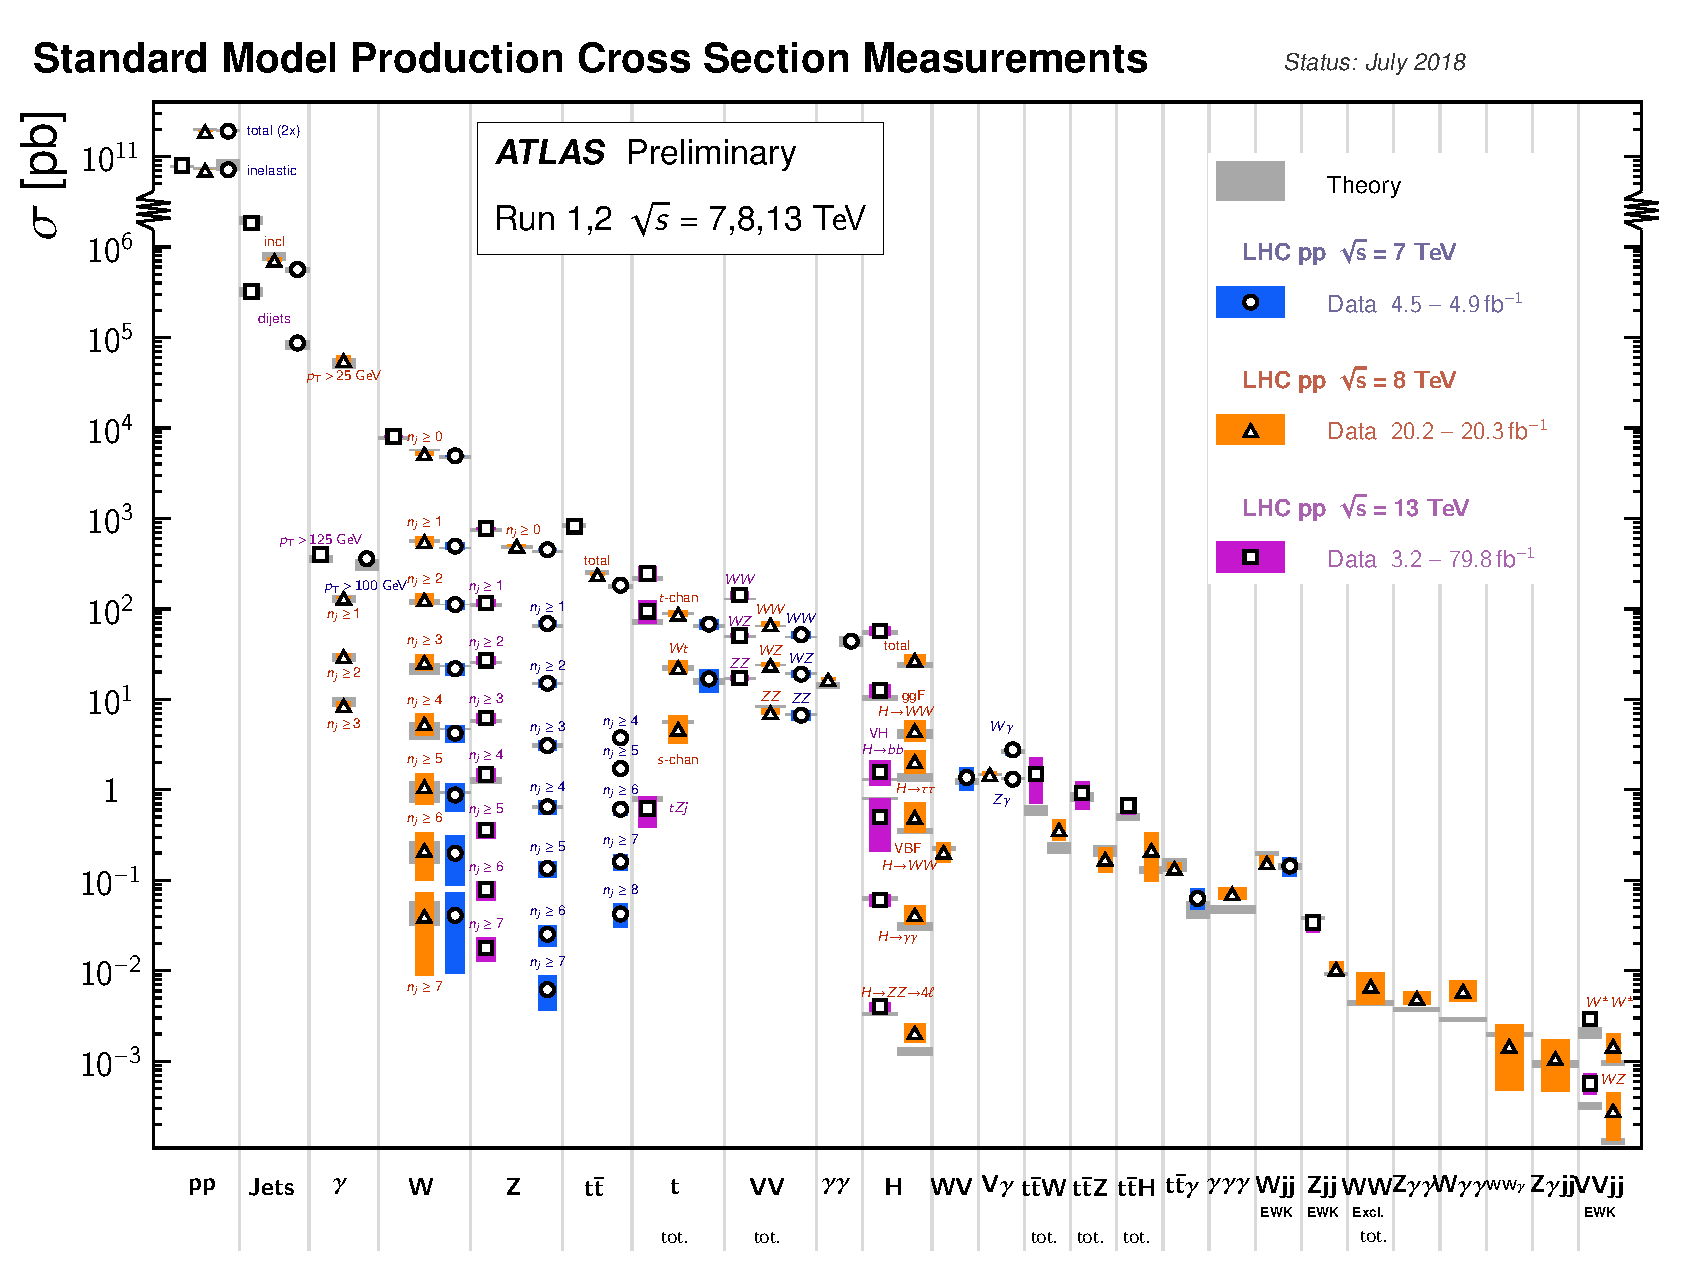
\includegraphics[width=\hsize]{figures/Theory/SM_xs.pdf}
  \caption{A comparison of cross section measurements at $\sqrt{s}=7,8,13$ TeV from ATLAS compared to theoretical measurements. From Ref. \cite{SM_XS_Comparison}}. 
  \label{fig:SM cross sections}
\end{figure}
\FloatBarrier


\chapter{New Physics Models with Diboson Resonances}
\label{BSM chapter}

\section{Randall Sundrum Bulk Model}
%Top down approach (solve gravity problem)
The electroweak-planck hierarchy may be explained by the existence of extra dimensions, like the 5D Randall Sundrum Bulk Model (\cite{rs2},\cite{rs1}). In this model, there is one extra warped spatial dimension, y, with a metric:
\begin{equation}
ds^{2}=e^{-2k|y|}\eta_{\mu\nu}dx^{\mu}dx^{\nu}+dy^{2} 
\end{equation}
where $e^{-k|y|}$ is the warp factor of the extra dimension, which is compactified on a $S^{1}/Z_{2}$ orbifold (a.k.a. a circle where $y \rightarrow -y$). This can be visualized as every point in space time having a line extending from it a distance L, representing this fifth dimension. At the end of this line is the Planck brane. This fourth spatial dimension separates two 4-D branes: Planck brane and TeV brane. We live on the TeV brane, as shown in Figure ~\ref{fig:RS_cartoon}. The Higgs field (and to a lesser degree the top quark and graviton fields) is localized near the TeV Brane, while the light fermion fields are localized more near the Planck brane. Fundamental parameters are set on the Planck brane. The warp factor may be scaled away from all dimensionless SM terms by field redefinitions. However, the only dimensionful parameter, $m_{H}^{2}=v^{2}$ is rescaled by $\tilde{v}\sim e^{-kL}M_{Pl}\sim 1$TeV for $kL\sim 35$, explaining why gravity is so weak on the TeV brane. Also, by localizing the light fermion fields near the Planck brane and top and graviton fields near the TeV brane, the light quarks will have smaller masses. 

The two free parameters of this theory are $M_{PL}$ and $k$. Based on this RS Bulk model, all SM particles should have Kaluza-Klein (KK) excitations. In particular, the graviton would have KK excitations that prefer to decay to WW or ZZ, which is why this analysis searches for RS Gravitons. 


\begin{figure}[h!]
  \centering
  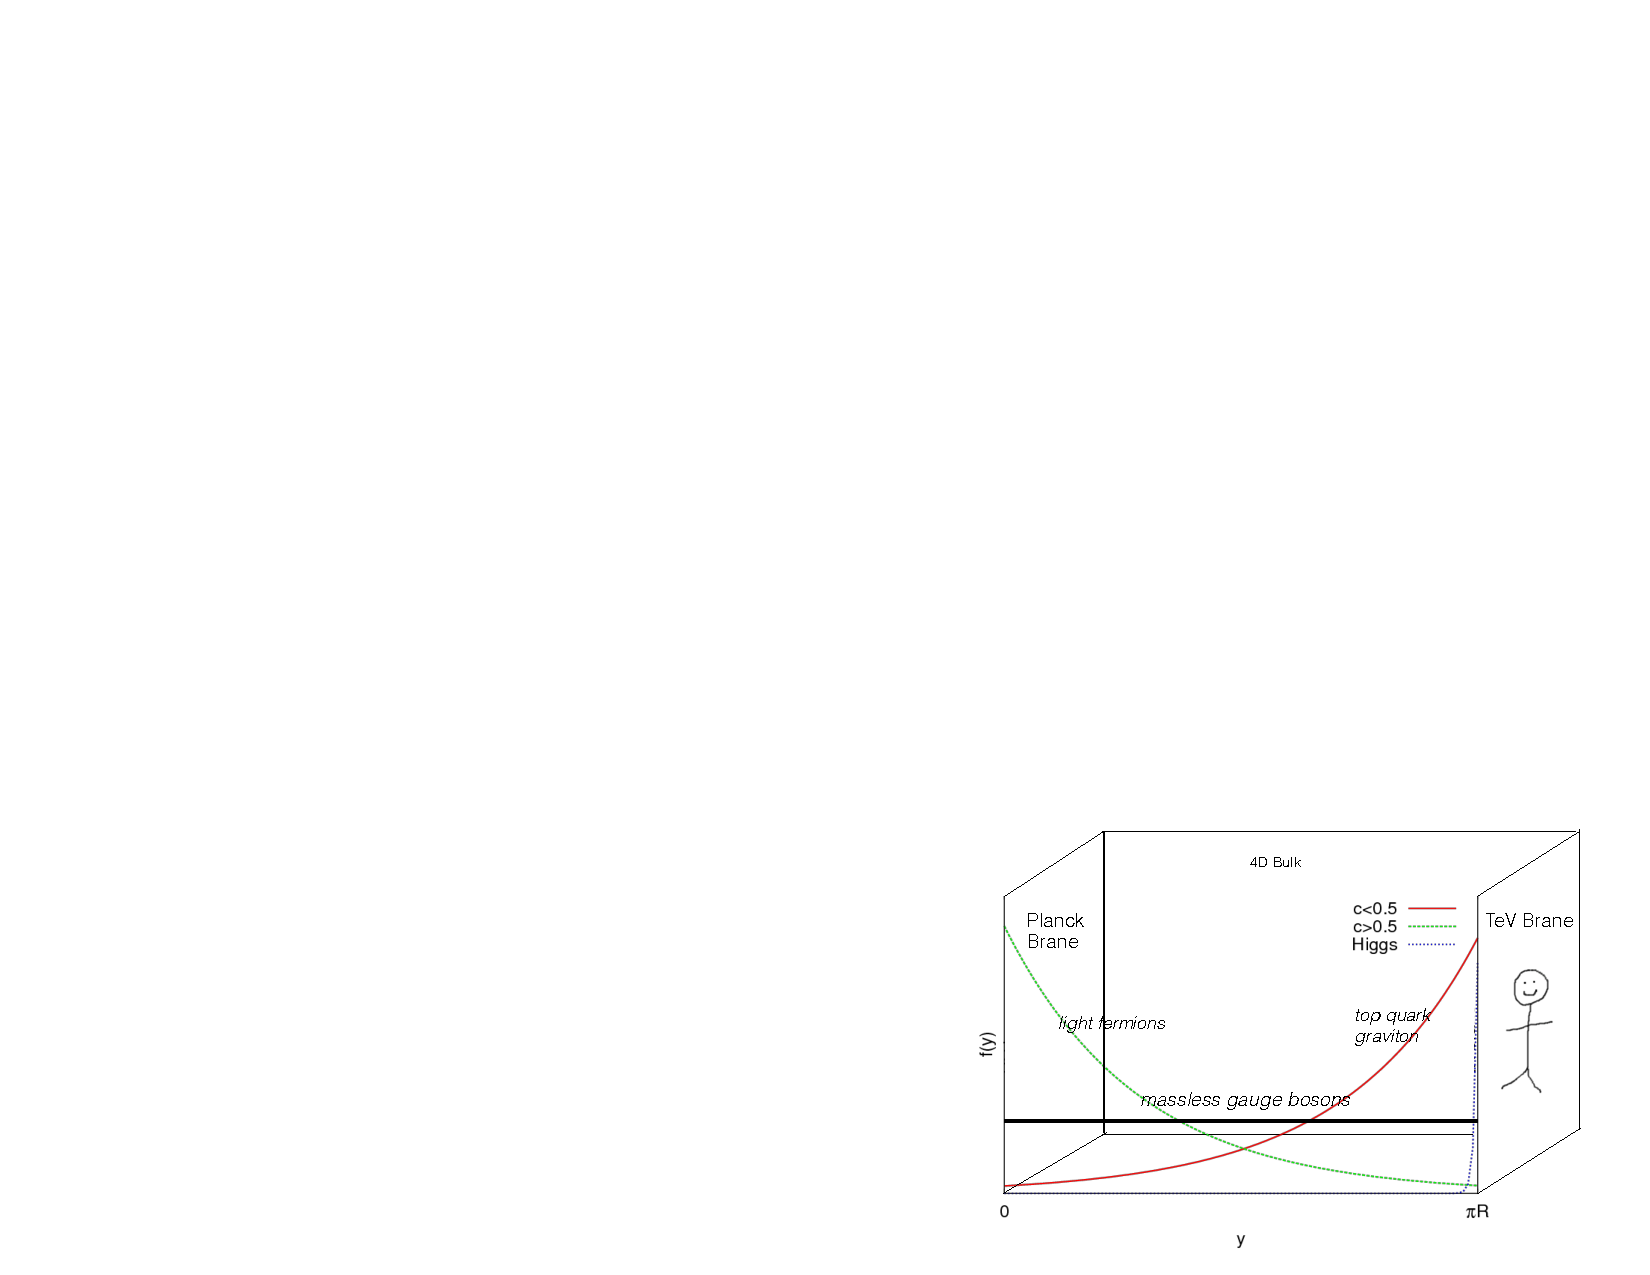
\includegraphics[width=\hsize]{figures/Theory/RS_cartoon.pdf}
  \caption{Cartoon of RS Bulk Model}. 
  \label{fig:RS_cartoon}
\end{figure}
\FloatBarrier

\begin{comment}
\section{Extended Scalar Sector}
%tries to solve physics problem but also somewhat ad-hoc (just a parameterization)
A further striking asymmetry of the SM is the simplicity of the scalar sector in comparison to the boson and fermion sectors. To date, the scalar sector has only one member, the Higgs boson. Therefore, it is natural to posit an extension to the scalar sector. From a theoretical standpoint this could also help generate baryon asymmetry through additional sources of CP violation. This analysis searches for a simple extension to the scalar sector as proposed in Ref. \cite{scalarsinglet}. The extended scalar sector includes a real Higgs singlet (S) and complex $SU(2)_{L}$ doublet ($\Phi$) (the SM Higgs), where mass eigenstates are mixtures of the fields. S has a vev of $v$ and $\Phi$ has a vev of $x$. This then gives a Lagrangian of:

\begin{equation}
\mathcal{L}\supset (D^{\mu}\Phi)^{\dag}D_{\mu}\Phi + \partial^{\mu}S\partial_{\mu}S - m^{2}\Phi^{\dag}\Phi-\mu^{2}S^{2} + \lambda_{1}(\Phi^{\dag}\Phi)^{2} + \lambda_{2}S^{4}+\lambda_{3}\Phi^{\dag}\Phi S^{2}
\end{equation}


The mass eigenstates of the scalar sector are then mixtures of $S$ and $\Phi$ and the free parameters of the theory are $m_{H}$, $\sin\alpha$, and $tan\beta=v/x$. The fields are then given by:

\begin{equation}
\Phi \equiv \begin{pmatrix} 0 \\ \frac{\tilde{h}+v}{\sqrt{2}} \end{pmatrix}
\end{equation}
\begin{equation}
S \equiv \frac{h'+x}{\sqrt{2}}
\end{equation}

Diagonalizing the mass matrix leads to the mass eigenstates h (discovered Higgs boson) and H (the physical particles):

\begin{equation}
\begin{pmatrix} h \\ H \end{pmatrix} = \begin{pmatrix} \cos\alpha &-\sin\alpha \\ \sin\alpha & \cos\alpha \end{pmatrix}
\end{equation}
This suppressed h and H production and SM H couplings:

\begin{equation}
BR_{H \rightarrow SM}=\sin^{2}\alpha \times \frac{\Gamma_{SM, H \rightarrow SM}}{\Gamma_{tot}}
\end{equation}
Moreover, in the case that $m_{H} > m_{h}$, $H\rightarrow hh$ is possible. This further suppresses $H \rightarrow VV/ff$. This search is most sensitive to $H \rightarrow WW$.
\end{comment}

\section{Simple Standard Model Extensions}
\label{HVT chapter}
The RS Bulk model is motivated by resolving SM hierarchies, but it does not address all of the other SM issues. There are many other interesting and well motivated new physics frameworks that address these issues, but there is a lack of completely predictive models, due to model flexibility (free parameters). It is difficult for experimentalists to know which theories to search for in data. Therefore, developing a model-independent resonance search that can be reinterperted in the context of a given BSM theory is ideal.

This search is sensitive to the resonance mass and its interactions, but not all of a given BSM model's parameters. Therefore, the BSM Lagrangian may be reduced to only retain this information (mass parameters and couplings) following the procedure in \cite{hvt}.
In this simplified approach, the new resonance searched for is represented as an additional heavy vector triplet (HVT), which is a real vector field in the adjoint representation of $SU(2)_{L}$ with vanishing hypercharge. This results in one neutral and two charged bosons, defined as:

\begin{equation}
V^{\pm}=\frac{V^{1}_{\mu}\mp iV^{2}_{\mu}}{\sqrt{2}}
\end{equation}
\begin{equation}
V^{0}_{\mu}=V^{3}_{\mu}
\end{equation}

The SM Lagrangian is then augmented with the additional terms:
\begin{equation}
\label{hvt_lagrangian}
\mathcal{L}\supset -\frac{1}{4}D_{[\mu}V^{a}_{\nu]}D^{[\mu}V^{\mu]a} + \frac{m_{V}^{2}}{2}V^{a}_{\mu}V^{a\mu} + ig_{V}c_{H}V^{a}_{\mu}H^{\dag}\tau^{a}\overset\leftrightarrow{D^{\mu}}H+\frac{g^{2}}{g_{V}}c_{F}V^{a}_{\mu}J_{F}^{\mu a}
\end{equation}


In order the terms represent: the kinetic, $V$ mass, Higgs-$V$ interaction, and $V$-left-handed fermion interaction terms. The $g_{V}$ coupling factor determines the coupling of the new resonance to left-handed fermions and the Higgs boson. 

As benchmark models, this search considers resonances from extended gauge symmetry (EGM) and composite Higgs models as discussed in \cite{hvt} . The EGM model predicts weakly coupled resonances, where $g_{V} = 1$, referred to later as Model A. The composite Higgs Model is a strongly coupled model, where $g_{V}=3$, and later referred to as Model B. 
As shown in Eq. \ref{hvt_lagrangian}, the coupling of these resonances to fermions scales as $g_{f} = g^{2}c_{F}/g_{V}$, where g is the SM $SU(2)_{L}$ gauge coupling and $c_{F}$ is a free parameter. This then means that for Model B the coupling to fermions is suppressed relative to Model A, leading to a smaller DY production rate and branching ratio (BR) to fermionic final states. The coupling of $V$ to SM bosons scales as $g_{H}=g_{V}c_{H}$, where $c_{H}$ is a free parameter on the order of one for Model A and B. Consequently Model A resonances have a smaller the BR to gauge bosons than Model B. For the $pp$ collision data used, Model A predicts larger production cross sections decaying to leptons and fermions than Model B which decays primarily to gauge bosons.

Model A and B vectors are produced via quark-anti-quark annihilation and the more rare vector-boson-fusion is considered by setting $g_{H} = 1$ and $g_{F}=0$. Both production modes are probed in this resonance search. 

In summary, $V$ couples most strongly to left-handed fermions and $VV$ dependent on $g_{V}$. 
